% -- coding: utf-8 --
\documentclass[a4paper, 11pt]{article}

% --- Podstawowe pakiety ---
\usepackage[utf8]{inputenc}      % Kodowanie UTF-8
\usepackage[T1]{fontenc}         % Kodowanie czcionek (ważne dla polskich znaków)
\usepackage[polish]{babel}       % Język polski (dzielenie wyrazów, nazwy)
\usepackage{amsmath}             % Pakiety matematyczne AMS
\usepackage{amssymb}             % Dodatkowe symbole matematyczne (np. dla normy)
\usepackage{graphicx}            % Dołączanie grafiki
\usepackage{geometry}            % Ustawienia marginesów
\usepackage{float}               % Lepsze zarządzanie obiektami pływającymi (np. [H] - here)
\usepackage{hyperref}            % Tworzenie hiperłączy (np. w spisie treści, do bibliografii)
\usepackage{siunitx}             % Ładne formatowanie liczb i jednostek (np. notacja naukowa)
\usepackage{booktabs}            % Ładniejsze linie w tabelach
\usepackage{listings}            % Do wstawiania kodu (jeśli potrzebne)
\usepackage{xcolor}              % Kolory (np. dla kodu)

% --- Ustawienia strony ---
\geometry{a4paper, left=2.5cm, right=2.5cm, top=2.5cm, bottom=2.5cm}

% --- Ustawienia formatowania liczb ---
\sisetup{
output-decimal-marker={,}, % Używaj przecinka jako separatora dziesiętnego
exponent-product=\cdot,   % Znak mnożenia dla notacji naukowej
scientific-notation=true,
round-mode=places,         % Tryb zaokrąglania
round-precision=4          % Liczba miejsc po przecinku dla czasów
}

% Definicja normy
\newcommand{\norm}[1]{\left\lVert#1\right\rVert}

% Ustawienia dla listings (opcjonalne, jeśli chcemy wstawiać kod)
\lstset{
    basicstyle=\ttfamily\small,
    keywordstyle=\color{blue},
    commentstyle=\color{green!50!black},
    stringstyle=\color{red},
    breaklines=true,
    showstringspaces=false,
    numbers=left,
    numberstyle=\tiny\color{gray},
    frame=single,
    inputencoding=utf8 % Ważne dla polskich znaków w kodzie
}

% --- Tytuł ---
\title{Metody Numeryczne - Projekt 2 \ Układy Równań Liniowych}
\author{Yauheni Pyryeu 201253}
\date{13 maja 2025} 

\begin{document}

\maketitle

\section{Wstęp}
Projekt niniejszy koncentruje się na implementacji i analizie porównawczej metod rozwiązywania układów równań liniowych postaci $Ax = b$. Rozważono dwie kategorie metod: iteracyjne, obejmujące metodę Jacobiego oraz Gaussa–Seidla, a także metodę bezpośrednią opartą na faktoryzacji LU. Szczególną uwagę zwrócono na potencjalne optymalizacje wynikające z pasmowej struktury macierzy $A$. Badania przeprowadzono w środowisku Python, wykorzystując biblioteki NumPy do obliczeń numerycznych oraz Matplotlib do wizualizacji wyników.

\section{Konstrukcja układu równań}
Parametry definiujące układ równań zostały ustalone na podstawie numeru indeksu studenta: \textbf{201253}. Poszczególne cyfry indeksu wykorzystano w następujący sposób:
\begin{itemize}
    \item Przedostatnia cyfra indeksu: $c = 5$
    \item Ostatnia cyfra indeksu: $d = 3$
    \item Czwarta cyfra indeksu: $e = 2$
    \item Trzecia cyfra indeksu: $f = 1$
\end{itemize}
Rozmiar macierzy kwadratowej $A$, oznaczony jako $N$, obliczono zgodnie ze wzorem: $N = 1200 + 10c + d = 1200 + 10 \cdot 5 + 3 = 1253$.

Macierz $A$ jest macierzą pięcioprzekątniową, a wartości na jej przekątnych są zdefiniowane następująco:
\begin{itemize}
    \item Główna przekątna ($a_{ii}$): wartość $a_1$. W zadaniach B (analiza zbieżności metod iteracyjnych) oraz E (analiza wydajności) przyjęto $a_1 = 5 + e = 5 + 2 = 7$. Natomiast w zadaniach C (badanie zbieżności dla innej macierzy) i D (metoda LU) $a_1 = 3$.
    \item Pierwsza podprzekątna ($a_{i, i-1}$) i nadprzekątna ($a_{i, i+1}$): $a_2 = -1$.
    \item Druga podprzekątna ($a_{i, i-2}$) i nadprzekątna ($a_{i, i+2}$): $a_3 = -1$.
\end{itemize}
Elementy wektora prawej strony $b$ (o długości $N$) są generowane za pomocą funkcji trygonometrycznej: $b_n = \sin(n(f+1)) = \sin(2n)$, gdzie $n = 1, 2, \dots, N$.

Celem jest wyznaczenie wektora $x$, który jest rozwiązaniem równania macierzowego $Ax = b$.

\section{Implementacja Algorytmów}
Wszystkie algorytmy zaimplementowano w języku Python 3. Do operacji na macierzach i wektorach, takich jak ich tworzenie, mnożenie czy obliczanie normy, wykorzystano bibliotekę NumPy. Wykresy ilustrujące wyniki zostały wygenerowane przy użyciu biblioteki Matplotlib. Pomiary czasu wykonania poszczególnych metod realizowano za pomocą funkcji \texttt{time.perf\_counter()}.

\subsection{Metody Iteracyjne (Jacobi, Gauss-Seidel)}
Implementacja metod iteracyjnych została przeprowadzona ręcznie. Macierz $A$ była generowana i przechowywana jako standardowa, gęsta macierz NumPy, mimo jej pasmowej natury.
W przypadku \textbf{metody Jacobiego}, implementacja wykorzystuje operacje na macierzach NumPy. Macierz $R = A - D$ (gdzie $D$ to macierz diagonalna $A$) jest tworzona jawnie, a następnie używana w operacji mnożenia macierzy przez wektor $R \cdot x^{(k)}$. Chociaż macierz $R$ jest również pasmowa, standardowe operacje NumPy niekoniecznie wykorzystują tę strukturę w sposób maksymalnie efektywny pod kątem unikania obliczeń na elementach zerowych.
Natomiast \textbf{metoda Gaussa–Seidla} została zaimplementowana z wykorzystaniem pętli, które iterują po elementach macierzy $A$ i wektora $x$. W każdej iteracji, przy obliczaniu nowej wartości $x_i^{(k+1)}$, odwołania do elementów macierzy $A$ ograniczają się jedynie do tych znajdujących się na niezerowych pasmach. Stanowi to optymalizację na poziomie operacyjnym, dostosowaną do pięcioprzekątniowej struktury macierzy.

Kryterium zakończenia iteracji dla obu metod było dwojakie: osiągnięcie normy residuum $r = \norm{Ax - b}$ mniejszej niż $10^{-9}$ lub przekroczenie maksymalnej liczby 2000 iteracji.

\subsection{Metoda Bezpośrednia (Faktoryzacja LU)}
Metoda bezpośrednia, oparta na dekompozycji LU, została zaimplementowana przy użyciu standardowych, gęstych macierzy NumPy.
\textbf{Faktoryzacja LU:} Zaimplementowano funkcję dokonującą rozkładu macierzy $A$ na iloczyn macierzy dolnotrójkątnej $L$ (z elementami jednostkowymi na głównej przekątnej) oraz macierzy górnotrójkątnej $U$, czyli $A = LU$.
Po uzyskaniu macierzy $L$ i $U$, rozwiązanie układu $Ax=b$ sprowadza się do rozwiązania dwóch prostszych układów równań z macierzami trójkątnymi: najpierw $Ly=b$ metodą podstawiania w przód, a następnie $Ux=y$ metodą podstawiania wstecz.

\section{Metody iteracyjne Jacobiego i Gaussa–Seidla}

\subsection{Formuły Metod Iteracyjnych}
Rozważmy układ równań $Ax=b$. Metody iteracyjne rozpoczynają obliczenia od pewnego początkowego przybliżenia rozwiązania $x^{(0)}$ i w kolejnych krokach generują ciąg przybliżeń $x^{(k)}$, który w założeniu ma zbiegać do faktycznego rozwiązania $x$.

\textbf{Metoda Jacobiego:} W $(k+1)$-tej iteracji, $i$-ta składowa wektora $x$ jest obliczana na podstawie wartości wszystkich składowych wektora $x^{(k)}$ pochodzących z poprzedniej, $k$-tej iteracji:
\begin{equation}
x_i^{(k+1)} = \frac{1}{a_{ii}} \left( b_i - \sum_{j=1, j \neq i}^{N} a_{ij} x_j^{(k)} \right)
\end{equation}
Dla analizowanej macierzy pięcioprzekątniowej (gdzie $a_{ii}=a_1$, $a_{i,i\pm 1}=a_2$, $a_{i,i\pm 2}=a_3$), przy uwzględnieniu jedynie niezerowych pasm, wzór ten przyjmuje postać (pomijając wyrazy spoza macierzy dla skrajnych indeksów $i$):
\begin{equation}
x_i^{(k+1)} = \frac{1}{a_1} \left( b_i - a_3 x_{i-2}^{(k)} - a_2 x_{i-1}^{(k)} - a_2 x_{i+1}^{(k)} - a_3 x_{i+2}^{(k)} \right)
\label{eq:jacobi_sparse}
\end{equation}

\textbf{Metoda Gaussa–Seidla:} W tej metodzie, podczas obliczania $i$-tej składowej $x_i^{(k+1)}$ w $(k+1)$-tej iteracji, wykorzystywane są już nowo obliczone w tej samej iteracji składowe $x_j^{(k+1)}$ dla $j < i$, oraz składowe $x_j^{(k)}$ z poprzedniej iteracji dla $j > i$:
\begin{equation}
x_i^{(k+1)} = \frac{1}{a_{ii}} \left( b_i - \sum_{j=1}^{i-1} a_{ij} x_j^{(k+1)} - \sum_{j=i+1}^{N} a_{ij} x_j^{(k)} \right)
\end{equation}
Dla badanej macierzy pięcioprzekątniowej wzór ten, po uwzględnieniu jej struktury, wygląda następująco:
\begin{equation}
x_i^{(k+1)} = \frac{1}{a_1} \left( b_i - a_3 x_{i-2}^{(k+1)} - a_2 x_{i-1}^{(k+1)} - a_2 x_{i+1}^{(k)} - a_3 x_{i+2}^{(k)} \right)
\label{eq:gauss_seidel_sparse}
\end{equation}

\subsection{Wyniki dla $a_1=7$}
Dla układu równań z $N=1253$ oraz wartością $a_1=7$ na głównej przekątnej (przy $a_2=a_3=-1$), uzyskano następujące wyniki. Kryterium stopu było osiągnięcie normy residuum $r < 10^{-9}$ lub wykonanie 2000 iteracji.
\begin{itemize}
    \item \textbf{Metoda Jacobiego:}
    \begin{itemize}
        \item Liczba iteracji: 30
        \item Czas wykonania: \num{0.0128} s
        \item Końcowa norma residuum: \num{6.026178341430422e-10}
    \end{itemize}
    \item \textbf{Metoda Gaussa–Seidla:}
    \begin{itemize}
        \item Liczba iteracji: 20
        \item Czas wykonania: \num{0.0517} s
        \item Końcowa norma residuum: \num{6.974854848483507e-10}
    \end{itemize}
\end{itemize}
Macierz dla $a_1=7$ jest silnie diagonalnie dominująca wierszowo ($|7| > |-1|+|-1|+|-1|+|-1|$), co jest warunkiem wystarczającym dla zbieżności obu metod iteracyjnych. Zgodnie z oczekiwaniami, metoda Gaussa–Seidla wymagała mniejszej liczby iteracji do osiągnięcia zadanej tolerancji niż metoda Jacobiego. Interesujące jest jednak, że całkowity czas wykonania metody Gaussa–Seidla był dłuższy. Może to wynikać z faktu, iż jej implementacja opierała się na pętlach Pythona, podczas gdy metoda Jacobiego, mimo potencjalnie większej liczby operacji arytmetycznych na skutek operowania na pełniejszej macierzy $R$, korzystała w większym stopniu ze zoptymalizowanych operacji wektorowych NumPy. Przebieg zbieżności obu metod zilustrowano na Rysunku \ref{fig:task_b_convergence}.

\begin{figure}[H]
    \centering
    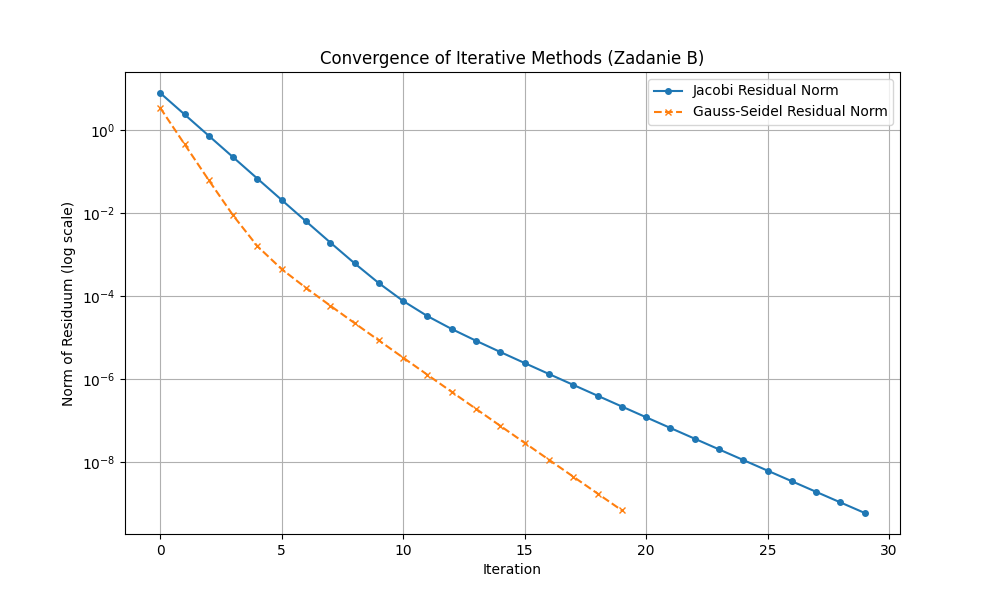
\includegraphics[width=0.8\textwidth]{residuals_plot_B}
    \caption{Zmiana normy residuum w kolejnych iteracjach dla metod Jacobiego i Gaussa–Seidla ($N=1253, a_1=7$).}
    \label{fig:task_b_convergence}
\end{figure}

\section{Analiza zbieżności dla $a_1 = 3$}
Zmiana wartości na głównej przekątnej na $a_1=3$ (przy $a_2=a_3=-1$) prowadzi do sytuacji, w której macierz $A$ przestaje być diagonalnie dominująca. Dla $i$-tego wiersza mamy bowiem $|a_{ii}| = |3| = 3$, podczas gdy suma modułów pozostałych elementów w tym wierszu (dla wierszy wewnętrznych) wynosi $|-1|+|-1|+|-1|+|-1| = 4$. Ponieważ $3 < 4$, warunek dominacji diagonalnej nie jest spełniony. Zbadano zachowanie metod iteracyjnych dla tak zmodyfikowanej macierzy, utrzymując limit 2000 iteracji.

Uzyskane rezultaty:
\begin{itemize}
    \item \textbf{Metoda Jacobiego:} nie osiągnęła zbieżności w ramach 2000 iteracji. Czas wykonania wyniósł \num{4.4741} s, a końcowa norma residuum osiągnęła wartość $\inf$, wskazując na dywergencję.
    \item \textbf{Metoda Gaussa–Seidla:} również nie zbiegła po 2000 iteracjach. Czas obliczeń to \num{5.6585} s. Końcowa norma residuum osiągnęła wartość NaN (Not a Number), co świadczy o niestabilności numerycznej i rozbieżności tej metody dla badanego przypadku.
\end{itemize}
Brak dominacji diagonalnej macierzy $A$ (dla $a_1=3$) skutkował rozbieżnością obu zastosowanych metod iteracyjnych. Przebieg zmian normy residuum w funkcji liczby iteracji dla tego przypadku przedstawiono na Rysunku~\ref{fig:task_c_convergence}.

\begin{figure}[H]
    \centering
    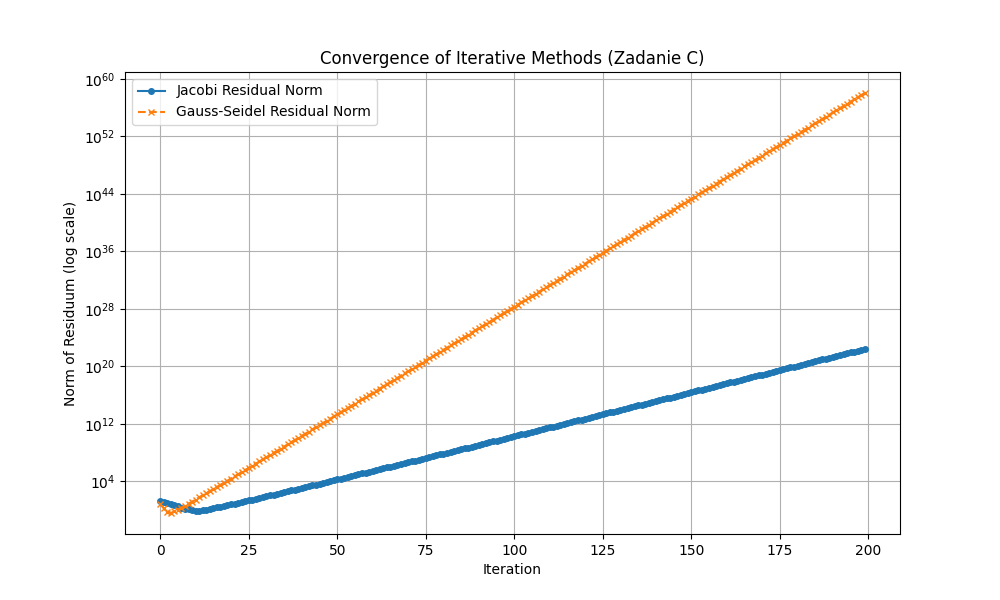
\includegraphics[width=0.8\textwidth]{residuals_plot_C}
    \caption{Zmiana normy residuum w kolejnych iteracjach dla metod Jacobiego i Gaussa–Seidla ($N=1253, a_1=3$).}
    \label{fig:task_c_convergence}
\end{figure}

\section{Metoda bezpośrednia}
Wobec niepowodzenia metod iteracyjnych w rozwiązaniu układu równań z macierzą $A$ dla $a_1=3$, zastosowano metodę bezpośrednią opartą na dekompozycji LU.

\subsection{Zasady Działania Metody Bezpośredniej LU}
Metoda ta polega na przedstawieniu macierzy $A$ jako iloczynu dwóch macierzy trójkątnych: dolnotrójkątnej $L$ (z jedynkami na głównej przekątnej) i górnotrójkątnej $U$. Po dokonaniu rozkładu $A = LU$, pierwotny układ równań $Ax=b$ można przekształcić w $LUx=b$. Rozwiązanie tego problemu sprowadza się do rozwiązania dwóch prostszych układów:
\begin{enumerate}
    \item $Ly = b$: rozwiązywany metodą podstawiania w przód (forward substitution) w celu wyznaczenia wektora pomocniczego $y$.
    \item $Ux = y$: rozwiązywany metodą podstawiania wstecz (backward substitution) w celu wyznaczenia ostatecznego rozwiązania $x$.
\end{enumerate}

\subsection{Wyniki dla $a_1=3$, $N=1253$}
Dla układu z macierzą, która nie była diagonalnie dominująca ($a_1=3$), zastosowanie metody rozkładu LU pozwoliło uzyskać następujące wyniki:
\begin{itemize}
    \item Łączny czas wykonania (dekompozycja LU + rozwiązanie układów trójkątnych): \num{3.1408} s
    \item Końcowa norma residuum: \num{6.24e-13}
\end{itemize}
Metoda bezpośrednia umożliwiła uzyskanie rozwiązania o wysokiej dokładności (mała norma residuum). Warto jednak zauważyć, że czas jej wykonania był znacząco dłuższy w porównaniu do czasów zbieżnych metod iteracyjnych (prezentowanych w sekcji 4.2 dla $a_1=7$).

\section{Analiza wydajności w zależności od $N$}
W celu zbadania wpływu rozmiaru macierzy $N$ na czas wykonania, przeprowadzono serię testów dla wszystkich trzech zaimplementowanych metod (Jacobi, Gauss-Seidel, LU). W tej analizie wykorzystano macierz $A$ z parametrem $a_1=7$, dla której metody iteracyjne wykazywały zbieżność. Testy wykonano dla następujących wartości $N$: $\{100, 300, 900, 1200, 2000\}$. Wyniki czasowe zebrano w Tabeli \ref{tab:task_e_times} oraz przedstawiono graficznie na Rysunkach \ref{fig:task_e_linear} (skala liniowa osi Y) i \ref{fig:task_e_log} (skala logarytmiczna osi Y).

\begin{table}[H]
    \centering
    \caption{Czasy wykonania [s] dla różnych wartości $N$ ($a_1=7$).}
    \label{tab:task_e_times}
    \begin{tabular}{r S[table-format=1.4] S[table-format=1.4] S[table-format=1.4] S[table-format=1.4]}
        \toprule
        {$N$} & {Jacobi} & {Gauss--Seidel} & {LU} \\
        \midrule
        100  & 0.0005 & 0.0046 & 0.0014\\
        300  & 0.0007 & 0.0118 & 0.0062\\
        900  & 0.0093 & 0.0386 & 0.0635\\
        1200 & 0.0137 & 0.0544 & 0.1037\\
        2000 & 0.0486 & 0.0775 & 0.2923\\
        \bottomrule
    \end{tabular}
\end{table}

\begin{figure}[H]
    \centering
    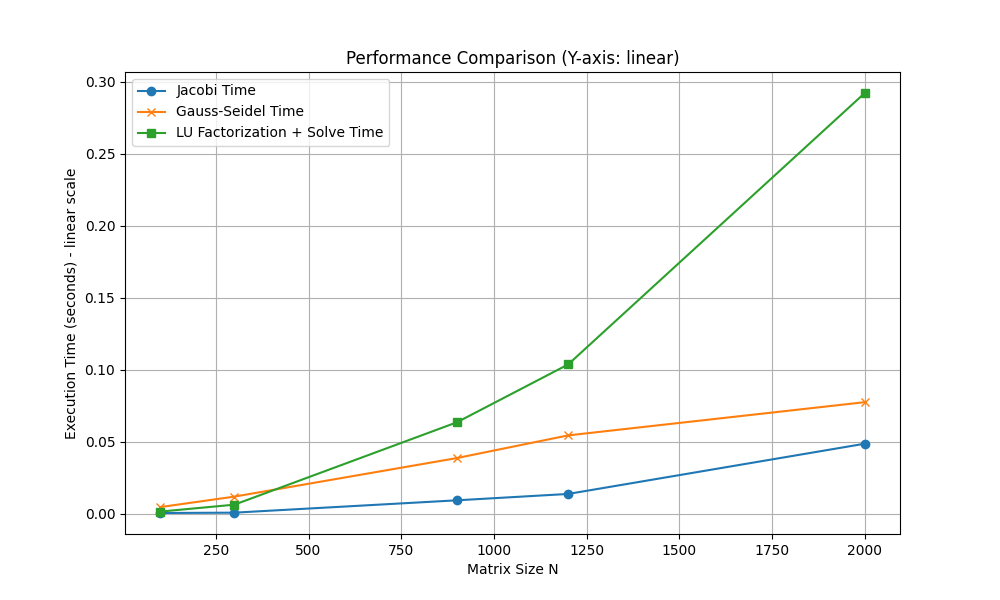
\includegraphics[width=0.8\textwidth]{performance_plot_linear_scale}
    \caption{Czas wykonania w zależności od $N$ dla wszystkich metod (skala liniowa osi Y).}
    \label{fig:task_e_linear}
\end{figure}

\begin{figure}[H]
    \centering
    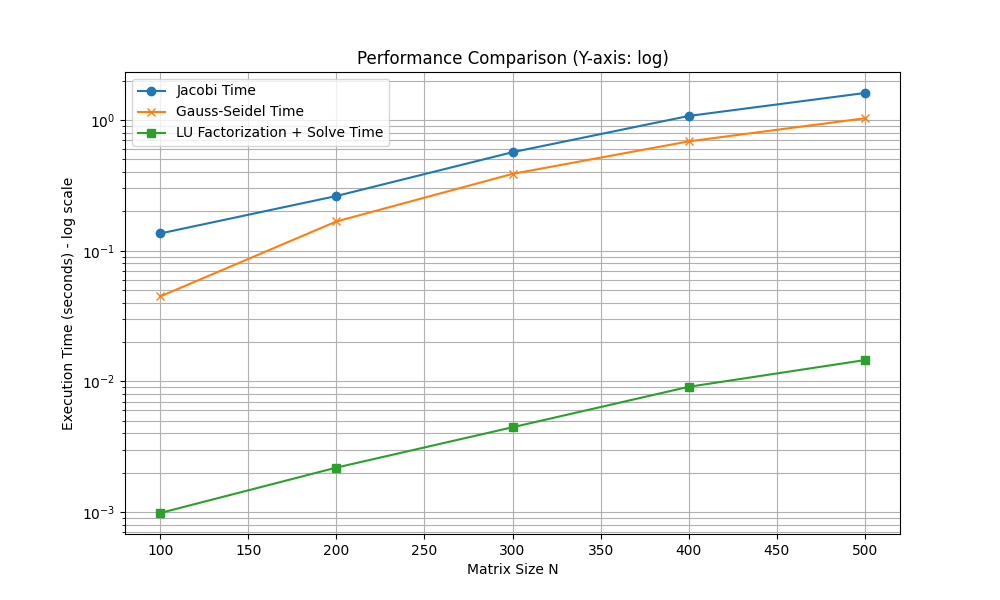
\includegraphics[width=0.8\textwidth]{performance_plot_log_scale}
    \caption{Czas wykonania w zależności od $N$ dla wszystkich metod (skala logarytmiczna osi Y).}
    \label{fig:task_e_log}
\end{figure}

\section{Wnioski}
Przeprowadzone eksperymenty i analiza wyników pozwalają sformułować następujące wnioski:
\begin{enumerate}
    \item \textbf{Zbieżność metod iteracyjnych:} Metody Jacobiego oraz Gaussa–Seidla wykazały zbieżność dla macierzy silnie diagonalnie dominującej (przypadek $a_1=7$). W sytuacji, gdy warunek ten nie był spełniony (przypadek $a_1=3$), obie metody okazały się rozbieżne. W przypadku zbieżności, metoda Gaussa–Seidla wymagała mniejszej liczby iteracji niż metoda Jacobiego. Niemniej jednak, dla $a_1=7$, całkowity czas obliczeń dla metody Gaussa-Seidla był dłuższy, co może być efektem różnic w implementacji – pętlowa struktura w Gaussie-Seidlu versus bardziej zwektoryzowane operacje NumPy w metodzie Jacobiego, nawet jeśli ta druga nie była w pełni zoptymalizowana pod kątem pasmowości.
    \item \textbf{Niezawodność metody bezpośredniej:} Metoda rozkładu LU pozwoliła na znalezienie rozwiązania niezależnie od tego, czy macierz $A$ była diagonalnie dominująca, czy nie. Charakteryzuje się ona większą niezawodnością w kontekście gwarancji uzyskania wyniku (o ile macierz jest nieosobliwa).
    \item \textbf{Wydajność a struktura macierzy i rozmiar problemu:} Dla macierzy o strukturze pasmowej i odpowiednio dużych rozmiarach $N$, metody iteracyjne (pod warunkiem ich zbieżności) mogą oferować znaczącą przewagę wydajnościową nad metodami bezpośrednimi operującymi na macierzach traktowanych jako gęste. Zaimplementowana metoda Gaussa-Seidla, dzięki jawnemu wykorzystaniu struktury pasmowej w pętlach, wykazała skalowanie kosztu pojedynczej iteracji bliskie $O(N)$. Metoda Jacobiego w przedstawionej implementacji, operująca na macierzy $R$, wykazała nieco gorsze empiryczne skalowanie czasu na iterację. Mimo to, dla większych wartości $N$ (np. $N \ge 900$), obie metody iteracyjne okazały się szybsze od zaimplementowanej metody LU. Dla małych $N$ (np. $N=100$), narzuty związane z implementacją (np. pętle Pythona w G-S) mogą wpływać na czasy tak, że np. metoda LU (lub nawet Jacobi) może być konkurencyjna lub szybsza od G-S. Teoretyczna złożoność obliczeniowa standardowej faktoryzacji LU dla macierzy gęstych to $O(N^3)$, podczas gdy koszt iteracji dla metod iteracyjnych na macierzach pasmowych jest znacznie niższy.
    \item \textbf{Dokładność i kryterium stopu:} Norma residuum stanowi użyteczne narzędzie do oceny dokładności uzyskanego rozwiązania oraz jako kryterium zakończenia obliczeń dla metod iteracyjnych. Metody te kończą działanie po osiągnięciu predefiniowanej tolerancji. Metody bezpośrednie, z założenia, dążą do uzyskania rozwiązania z dokładnością ograniczoną przez precyzję arytmetyki zmiennoprzecinkowej używanej w obliczeniach.
\end{enumerate}
Podsumowując, wybór optymalnej metody rozwiązania układu równań liniowych jest zależny od charakterystyki problemu. Dla dużych, pasmowych (lub ogólnie rzadkich) macierzy spełniających warunki zbieżności, metody iteracyjne są często preferowane ze względu na ich efektywność obliczeniową. W przypadkach ogólnych, lub gdy zbieżność metod iteracyjnych nie jest zapewniona, metody bezpośrednie stanowią bardziej niezawodny, choć potencjalnie bardziej kosztowny obliczeniowo, wybór.

\end{document}